We first report the confirmatory comparison with trait-plus-autoregressive persistence, the eligibility of the other persistence comparisons, and the prespecified controls and sensitivities. The exploratory analyses then examine why the observed separation is fragile. Throughout, $a$ is a nominal innovation-variance fraction in the generator, not a directly interpretable intensity of social influence.

\subsection{Boundaries against trait-plus-autoregressive persistence}\label{sec:results-B}

All five recorded stages of the validation gate passed before any confirmatory seed was derived (\esmresource, Section~\ref{esm-sec:record-gate}), and all 414 units finished: \resultnum{v4.inv.n_valid}{342} complete and valid and \resultnum{j.inventory.invalid.total}{72} complete but invalid, of which \resultnum{j.inventory.invalid.c_related}{36} involve model C and \resultnum{j.inventory.invalid.anchoring_sensitivities}{36} are anchoring sensitivities (\esmresource, Section~\ref{esm-sec:inventory}; unit-level boundaries in \allunitsresource).

Figure~\ref{fig:auc-B} and Table~\ref{tab:boundaries-B} report the confirmatory comparison against trait-plus-autoregressive persistence (B). All nine B units were complete and valid, so the main curve is valid. The first boundary $a^*(r)$ was $a=\resultnum{j.b.r055.first.point}{0.10}$ at $r=0.55$ to $0.90$ and $a=\resultnum{j.b.r050.first.point}{0.30}$ at $r=0.50$. Every boundary interval lay entirely above $a=0.03$ and spanned at most one grid step, with a step only at $r=0.50$, $0.55$ and $0.60$. The sustained boundary $a^*_s(r)$ equaled the first at seven shares and is censored at $r=0.55$ and $0.70$ by fit gaps at the top of the grid, although the lower band stayed above $0.70$ at every available higher strength.

For a given matched model and trained rule, an AUC of $0.70$ means that a randomly drawn influence panel ranks above a randomly drawn persistence panel with probability $0.70$, counting ties as half. The target $\mathcal A(a,r)$ averages that ranking probability over the matching, validation and training procedure (Section~\ref{sec:methods-classifier}). Neither quantity is classification accuracy or power for a test on one panel, and neither identifies the cause of a difference. For equal-variance normal score distributions, an AUC of $0.70$ translates to single-panel power of about \resultnum{j.auc_translation.target070.power}{0.18} at a one-sided 5\% level against a known persistence score distribution (Table~\ref{tab:auc-translation}); this is an illustrative translation, not a measured rejection rate of the full fitting procedure.

\begin{figure*}[tp]
\centering
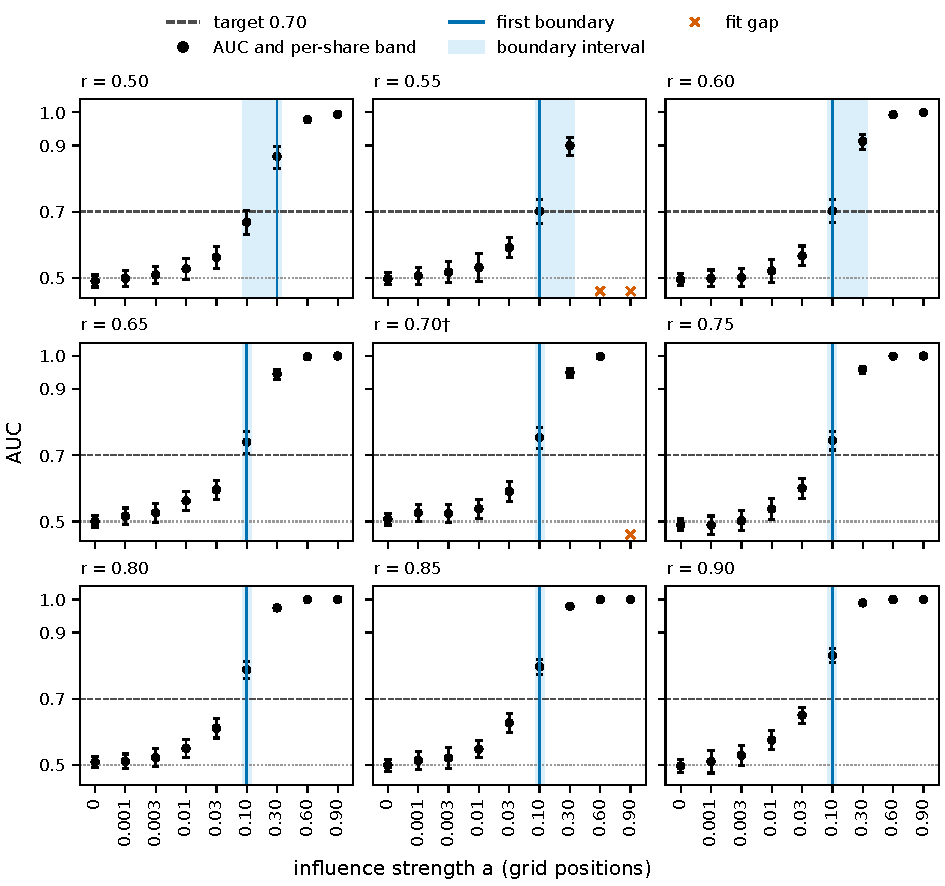
\includegraphics[width=\textwidth]{generated/J2_auc_profiles_B.pdf}
\caption{AUC profiles against trait-plus-autoregressive persistence (B), one panel per signal share $r$. Points are point AUCs; vertical bars show that share's band, simultaneous over strengths; the vertical line marks the first boundary and the shading its interval; crosses mark fit gaps. Dashed line: target \resultnum{j.target.r070}{0.70}. Dotted line: chance (\resultnum{j.chance}{0.5}). $\dag$ Examined during calibration.}\label{fig:auc-B}
\end{figure*}


\begin{table*}[tp]
\caption{Boundaries against trait-plus-autoregressive persistence (B).}\label{tab:boundaries-B}
\centering\scriptsize
\setlength{\tabcolsep}{5pt}
\begin{tabular}{l>{\raggedright\arraybackslash}p{22mm}>{\raggedright\arraybackslash}p{28mm}rrrrr}
\toprule
$r$ & $a^*$ [interval] & $a_s^*$ [interval] & \shortstack{AUC at\\\resultnum{j.grid.a0300}{0.03}} & \shortstack{AUC at\\\resultnum{j.grid.a1000}{0.10}} & \shortstack{AUC at\\\resultnum{j.grid.a3000}{0.30}} & \shortstack{Target\\\resultnum{j.target.r060}{0.60}} & \shortstack{Target\\\resultnum{j.target.r080}{0.80}} \\
\midrule
\resultnum{v4.tab.T1.B.r050.r}{0.50} & \resultnum{j.b.r050.first.point}{0.30} [\resultnum{j.b.r050.first.lower}{0.10}, \resultnum{j.b.r050.first.upper}{0.30}] & \resultnum{j.b.r050.sustained.point}{0.30} [\resultnum{j.b.r050.sustained.lower}{0.10}, \resultnum{j.b.r050.sustained.upper}{0.30}] & \resultnum{j.b.r050.a0300.auc}{0.562} & \resultnum{j.b.r050.a1000.auc}{0.668} & \resultnum{j.b.r050.a3000.auc}{0.867} & \resultnum{j.b.r050.target060.point}{0.10} & \resultnum{j.b.r050.target080.point}{0.30} \\
\resultnum{v4.tab.T1.B.r055.r}{0.55} & \resultnum{j.b.r055.first.point}{0.10} [\resultnum{j.b.r055.first.lower}{0.10}, \resultnum{j.b.r055.first.upper}{0.30}] & censored (fit gaps at \resultnum{j.b.r055.sustained.gap.0.a}{0.60}, \resultnum{j.b.r055.sustained.gap.1.a}{0.90}) & \resultnum{j.b.r055.a0300.auc}{0.591} & \resultnum{j.b.r055.a1000.auc}{0.702} & \resultnum{j.b.r055.a3000.auc}{0.900} & \resultnum{j.b.r055.target060.point}{0.10} & \resultnum{j.b.r055.target080.point}{0.30} \\
\resultnum{v4.tab.T1.B.r060.r}{0.60} & \resultnum{j.b.r060.first.point}{0.10} [\resultnum{j.b.r060.first.lower}{0.10}, \resultnum{j.b.r060.first.upper}{0.30}] & \resultnum{j.b.r060.sustained.point}{0.10} [\resultnum{j.b.r060.sustained.lower}{0.10}, \resultnum{j.b.r060.sustained.upper}{0.30}] & \resultnum{j.b.r060.a0300.auc}{0.567} & \resultnum{j.b.r060.a1000.auc}{0.702} & \resultnum{j.b.r060.a3000.auc}{0.913} & \resultnum{j.b.r060.target060.point}{0.10} & \resultnum{j.b.r060.target080.point}{0.30} \\
\resultnum{v4.tab.T1.B.r065.r}{0.65} & \resultnum{j.b.r065.first.point}{0.10} [\resultnum{j.b.r065.first.lower}{0.10}, \resultnum{j.b.r065.first.upper}{0.10}] & \resultnum{j.b.r065.sustained.point}{0.10} [\resultnum{j.b.r065.sustained.lower}{0.10}, \resultnum{j.b.r065.sustained.upper}{0.10}] & \resultnum{j.b.r065.a0300.auc}{0.596} & \resultnum{j.b.r065.a1000.auc}{0.740} & \resultnum{j.b.r065.a3000.auc}{0.946} & \resultnum{j.b.r065.target060.point}{0.10} & \resultnum{j.b.r065.target080.point}{0.30} \\
\resultnum{v4.tab.T1.B.r070.r}{0.70}\dag{} & \resultnum{j.b.r070.first.point}{0.10} [\resultnum{j.b.r070.first.lower}{0.10}, \resultnum{j.b.r070.first.upper}{0.10}] & censored (fit gap at \resultnum{j.b.r070.sustained.gap.0.a}{0.90}) & \resultnum{j.b.r070.a0300.auc}{0.591} & \resultnum{j.b.r070.a1000.auc}{0.754} & \resultnum{j.b.r070.a3000.auc}{0.950} & \resultnum{j.b.r070.target060.point}{0.10} & \resultnum{j.b.r070.target080.point}{0.30} \\
\resultnum{v4.tab.T1.B.r075.r}{0.75} & \resultnum{j.b.r075.first.point}{0.10} [\resultnum{j.b.r075.first.lower}{0.10}, \resultnum{j.b.r075.first.upper}{0.10}] & \resultnum{j.b.r075.sustained.point}{0.10} [\resultnum{j.b.r075.sustained.lower}{0.10}, \resultnum{j.b.r075.sustained.upper}{0.10}] & \resultnum{j.b.r075.a0300.auc}{0.600} & \resultnum{j.b.r075.a1000.auc}{0.745} & \resultnum{j.b.r075.a3000.auc}{0.959} & \resultnum{v4.tab.T1sec.B.r075.a060.1}{0.03} & \resultnum{j.b.r075.target080.point}{0.30} \\
\resultnum{v4.tab.T1.B.r080.r}{0.80} & \resultnum{j.b.r080.first.point}{0.10} [\resultnum{j.b.r080.first.lower}{0.10}, \resultnum{j.b.r080.first.upper}{0.10}] & \resultnum{j.b.r080.sustained.point}{0.10} [\resultnum{j.b.r080.sustained.lower}{0.10}, \resultnum{j.b.r080.sustained.upper}{0.10}] & \resultnum{j.b.r080.a0300.auc}{0.611} & \resultnum{j.b.r080.a1000.auc}{0.788} & \resultnum{j.b.r080.a3000.auc}{0.975} & \resultnum{v4.tab.T1sec.B.r080.a060.1}{0.03} & \resultnum{j.b.r080.target080.point}{0.30} \\
\resultnum{v4.tab.T1.B.r085.r}{0.85} & \resultnum{j.b.r085.first.point}{0.10} [\resultnum{j.b.r085.first.lower}{0.10}, \resultnum{j.b.r085.first.upper}{0.10}] & \resultnum{j.b.r085.sustained.point}{0.10} [\resultnum{j.b.r085.sustained.lower}{0.10}, \resultnum{j.b.r085.sustained.upper}{0.10}] & \resultnum{j.b.r085.a0300.auc}{0.627} & \resultnum{j.b.r085.a1000.auc}{0.797} & \resultnum{j.b.r085.a3000.auc}{0.979} & \resultnum{v4.tab.T1sec.B.r085.a060.1}{0.03} & \resultnum{j.b.r085.target080.point}{0.30} \\
\resultnum{v4.tab.T1.B.r090.r}{0.90} & \resultnum{j.b.r090.first.point}{0.10} [\resultnum{j.b.r090.first.lower}{0.10}, \resultnum{j.b.r090.first.upper}{0.10}] & \resultnum{j.b.r090.sustained.point}{0.10} [\resultnum{j.b.r090.sustained.lower}{0.10}, \resultnum{j.b.r090.sustained.upper}{0.10}] & \resultnum{j.b.r090.a0300.auc}{0.650} & \resultnum{j.b.r090.a1000.auc}{0.831} & \resultnum{j.b.r090.a3000.auc}{0.990} & \resultnum{v4.tab.T1sec.B.r090.a060.1}{0.03} & \resultnum{j.b.r090.target080.point}{0.10} \\
\botrule
\end{tabular}
\par\smallskip\parbox{\linewidth}{$r$ is signal share in the continuous response before discretization. $a^*$: first boundary [interval from the band]; $a_s^*$: sustained boundary; censored: not declared across fit gaps. All \resultnum{j.b.first.large.n}{9} first-boundary intervals lie entirely above \resultnum{j.grid.a0300}{0.03}. AUC columns give point estimates; target columns give first boundaries at secondary targets. \dag{} Examined during calibration. Definitions: \esmresource, Table~\ref{esm-tab:glossary-terms}.}
\end{table*}


Two descriptive readings qualify this curve. The flat boundary hides a dependence on $r$ that the coarse grid absorbs: the AUC at $a=0.10$ ranged from \resultnum{j.b.a1000.auc.min}{0.668} at $r=\resultnum{j.b.a1000.auc.min.r}{0.50}$ to \resultnum{j.b.a1000.auc.max}{0.831} at $r=\resultnum{j.b.a1000.auc.max.r}{0.90}$, tending to rise with $r$, and at $r=0.55$ and $0.60$ it was \resultnum{j.b.r055.a1000.auc}{0.702} and \resultnum{j.b.r060.a1000.auc}{0.702}, close to the target, so the intervals there extend to $a=\resultnum{j.b.r055.first.upper}{0.30}$. The arms already differed at $a=0.03$, where every lower band exceeded $0.5$ (the lowest was \resultnum{j.b.r050.a0300.lower}{0.528}, at $r=0.50$) and every upper band stayed below $0.70$ (the highest was \resultnum{j.b.a0300.upper.max}{0.675}, at $r=\resultnum{j.b.a0300.upper.max.r}{0.90}$). The boundary therefore marks a performance target, not the first detectable difference; the conjunction of nine intervals above $0.03$ carries no joint error rate. These readings were made after the results became available. Point AUCs, band limits and critical values for all \resultnum{v4.protocol.grid_cells}{81} cells are in \esmresource, Tables~\ref{esm-tab:b-cells}--\ref{esm-tab:b-cells-part-c}.

\subsection{Eligibility of the other persistence comparisons}\label{sec:results-other}

Table~\ref{tab:other-models} summarizes the secondary persistence models, whose AUC profiles are in \esmresource, Figs.~\ref{esm-fig:auc-A}--\ref{esm-fig:auc-E}. Against autoregressive persistence (A) and mover--stayer persistence (E), all units were complete and valid, every first boundary was \resultnum{j.models.A.r055.first.point}{0.10} or \resultnum{j.models.A.r050.first.point}{0.30} with an interval above $0.03$, and every sustained boundary equaled the first or was censored by fit gaps at the top of the grid.

\begin{table*}[tp]
\caption{Boundaries against the other persistence models.}\label{tab:other-models}
\centering\scriptsize
\setlength{\tabcolsep}{4pt}
\begin{tabular}{ll>{\raggedright\arraybackslash}p{62mm}>{\raggedright\arraybackslash}p{54mm}}
\toprule
Model & $r$ & First boundary & Sustained boundary \\
\midrule
A & \resultnum{j.models.r050.r}{0.50} & \resultnum{j.models.A.r050.first.point}{0.30} & \resultnum{j.models.A.r050.sustained.point}{0.30} \\
A & \resultnum{j.models.r055.r}{0.55}--\resultnum{j.models.r090.r}{0.90} & \resultnum{j.models.A.r055.first.point}{0.10} & \resultnum{j.models.A.r055.sustained.point}{0.10} \\
C & All shares & Invalid: zero-strength AUC \resultnum{j.models.C.zero_auc.min}{1.000} & Suppressed \\
D & All shares & Censored at first gap: \resultnum{j.models.D.r055.first.censoring_gap.a}{0.10} at \resultnum{j.models.D.first_gap.a1000.family_limit.n}{7} shares (family limit on profile); \resultnum{j.models.D.r050.first.censoring_gap.a}{0.01} at $r=$ \resultnum{j.models.D.r050.r}{0.50} (other solver status); \resultnum{j.models.D.r060.first.censoring_gap.a}{0.003} at $r=$ \resultnum{j.models.D.r060.r}{0.60} (propagation gap) & Censored (fit gaps) \\
E & \resultnum{j.models.r050.r}{0.50}--\resultnum{j.models.r060.r}{0.60} & \resultnum{j.models.E.r050.first.point}{0.30} & \resultnum{j.models.E.r050.sustained.point}{0.30}; censored at $r=$ \resultnum{j.models.r055.r}{0.55} (fit gaps at \resultnum{j.models.E.r055.sustained.gap.0.a}{0.60}, \resultnum{j.models.E.r055.sustained.gap.1.a}{0.90}) \\
E & \resultnum{j.models.r065.r}{0.65}--\resultnum{j.models.r090.r}{0.90} & \resultnum{j.models.E.r065.first.point}{0.10} & \resultnum{j.models.E.r065.sustained.point}{0.10}; censored at $r=$ \resultnum{j.models.r070.r}{0.70} (fit gap at \resultnum{j.models.E.r070.sustained.gap.0.a}{0.90}) \\
\botrule
\end{tabular}
\par\smallskip\parbox{\linewidth}{$r$ is signal share in the continuous response before discretization. A: autoregressive; C: autoregressive with an altered response channel; D: state-dependent; E: mover--stayer. A and E group consecutive shares with the same first boundary; sustained-boundary exceptions are explicit. Unmarked entries are complete and valid; C is complete but invalid, so its boundaries are suppressed. Boundary and censoring definitions: \esmresource, Table~\ref{esm-tab:glossary-terms}; fit statuses: Table~\ref{esm-tab:glossary-states}.}
\end{table*}


All nine units of autoregressive persistence with an altered response channel (C) were complete but invalid. C has no zero-strength identity: it alters the response channel of the persistence arm only. The classifier separated the arms perfectly at zero strength, with a point AUC of \resultnum{j.models.C.zero_auc.min}{1.000} at every share. This failed the prespecified zero-strength eligibility check and suppressed C's boundaries. The failure reflects the channel asymmetry, not evidence about persistence or influence, and by itself establishes no implementation defect. Because the prespecified comparison across persistence models required every secondary unit to be complete and valid, that comparison was unavailable and its prespecified display of offsets between models was not produced. The valid units remain displayed without promoting or demoting a persistence model.

All nine units of state-dependent persistence (D) were complete and valid, but fit gaps censor every first and sustained boundary, beginning at seven shares at $a=0.10$, where B's boundary lies (Table~\ref{tab:other-models}). Of D's \resultnum{j.models.D.gaps.total}{38} gap cells, \resultnum{j.models.D.gaps.family_limit}{33}, including every gap at $a=0.10$, are family limits: the prespecified profile solver reached the edge of D's parameter box without an accepted match. It found no admissible match at $a=0.10$ or $0.30$, the strengths of B's first boundaries, at any share. These are limits of the declared matching procedure, not AUCs below the target or proof that no parameter in the box could match the moments (\esmresource, Section~\ref{esm-sec:additional-models}).

\subsection{Measurement controls and sensitivities}\label{sec:results-controls}

The measurement controls repeat the comparison on error-free responses, reusing the second persistence parameter of the observed fit (\esmresource, Table~\ref{esm-tab:controls}). Against B, the ordinal control, discretized without error ($r=1$), and the latent-rank control reached the target at $a=\resultnum{j.controls.ordinal_one.r050.first.point}{0.10}$ at every share; only the latent control, with neither error nor discretization, reached it at $a=\resultnum{j.controls.latent.r055.first.point}{0.03}$, at \resultnum{j.controls.latent.n_boundary_a0300}{8} shares. Removing response error while retaining ordinal allocation left the point boundary unchanged at design shares from $r=0.55$ to $0.90$, but at $r=0.50$ it fell from $a=\resultnum{j.b.r050.first.point}{0.30}$ to $a=\resultnum{j.controls.ordinal_one.r050.first.point}{0.10}$.

Of the \resultnum{j.sensitivity.n_pairs_compared}{63} complete and valid sensitivity units, \resultnum{j.sensitivity.n_region_differs}{8} differed from the main curve in whether the first boundary was declared with an interval entirely above $a=0.03$ (\esmresource, Section~\ref{esm-sec:additional-controls}). Without repulsion ($b=0$), the first boundary was \resultnum{j.sensitivity.b000.first.min}{0.03} to \resultnum{j.sensitivity.b000.first.max}{0.10} at every share, with intervals reaching down to \resultnum{j.sensitivity.b000.r080.sensitivity.lower}{0.03} at $r=0.80$ to $0.90$, so repulsion is not needed for detection; with persistent response style or panel conditioning in both arms, \resultnum{j.sensitivity.response_channel.n_same_region}{44} of \resultnum{v4.inv.t4.n_valid}{45} units kept the interval above $a=0.03$. With \resultnum{v4.protocol.steps}{24} updates per wave and the same per-step persistence, the annual process itself changes, as annual latent persistence without influence falls to $0.85^{24}$, close to zero; anchoring to the initial state, which B lacks, separated the arms without influence (zero-strength AUC \resultnum{j.sensitivity.omega025.zero_auc.min}{0.647} to \resultnum{j.sensitivity.omega025.zero_auc.max}{0.892} at the weakest anchoring) or could not be fitted, so it is uninformative about influence.

\subsection{Exploratory explanations of separation and fragility}\label{sec:results-exploratory}

Table~\ref{tab:exploratory} describes each exploratory analysis. All lie outside the confirmatory estimand; they examine the scale, sources and sensitivity of separation rather than independently confirming the main curve. The twin, variance and stress-test analyses were read when they finished and the others after the results became available; every comparison with the main curve is a later reading.

\begin{table*}[tp]
\caption{Exploratory analyses at a glance. All were declared before any confirmatory result, use seeds disjoint from the confirmatory ones and lie outside the confirmatory estimand. Ranges are minima and maxima over signal shares; the last column is a reading made after the results became available. Full results and definitions: Online Resource~1, Section~\ref{esm-sec:exploratory} and Table~\ref{esm-tab:glossary-terms}.}\label{tab:exploratory}
\centering\scriptsize
\setlength{\tabcolsep}{2.5pt}
\begin{tabular}{@{}p{0.10\textwidth}p{0.13\textwidth}p{0.285\textwidth}p{0.265\textwidth}p{0.17\textwidth}@{}}
\toprule
\raggedright Analysis & \raggedright Question & \raggedright What changes relative to the main design & \raggedright Main result & \raggedright Reading \tabularnewline
\midrule
\raggedright Mean-field twin & \raggedright Is the persistent input from fixed contacts needed? & \raggedright Influence term replaced by fresh Gaussian noise with its mean and variance given the own state: keeps the own-state effect, removes the persistent input, the dependence between people and the term's shape & \raggedright Arm against twin at $a=0.10$: AUC \resultnum{j.x1a.auc.a010.min}{0.623}--\resultnum{j.x1a.auc.a010.max}{0.716}; mean lag correlations differing by at most \resultnum{j.x1a.lag_difference.a010.max}{0.0056}, positive at every lag and growing with it. Twin against B: target reached only at $r=0.90$, at $a=\resultnum{j.x1b.r090.first.point}{0.30}$ & \raggedright Separation does not come from the own-state effect alone; not network-specific; may include the start-up transient \tabularnewline
\raggedright Variance explained by influence & \raggedright What does a nominal strength mean on a variance scale? & \raggedright Latent paths without response channel; partial $R^2$ of the standardized influence term for the next latent attitude beyond linear persistence & \raggedright Partial $R^2$ \resultnum{j.x2a.a003}{0.016}, \resultnum{j.x2a.a010}{0.054} and \resultnum{j.x2a.a030}{0.167} at $a=0.03$, $0.10$ and $0.30$; a natural cubic spline of the own state with five knots absorbed little of it & \raggedright Little latent variance at the boundary; per-step latent scale; spline result specific to that spline \tabularnewline
\raggedright Free signal share & \raggedright Does separation survive when B fits its signal share? & \raggedright B fits its signal share with its two parameters to lags 1--3; both contrasts classify on lags 4--5 only & \raggedright At the first boundary, AUC \resultnum{j.x3.known.auc.min}{0.668}--\resultnum{j.x3.known.auc.max}{0.858} with the share known and \resultnum{j.x3.free.auc.min}{0.534}--\resultnum{j.x3.free.auc.max}{0.585} with it free; fitted share \resultnum{j.x3.free.r_shift.min}{0.0011}--\resultnum{j.x3.free.r_shift.max}{0.0028} below the true one; free-share interval below $0.70$ where the known-share AUC reached it in \resultnum{j.x3.lost_crossings.n}{18} of \resultnum{j.x3.lost_crossings.cells}{21} cells at $a=0.10$--$0.60$ & \raggedright One fit, contributions not disentangled, absorbed most separation; sensitive to reliability in the third decimal; matching uncertainty omitted \tabularnewline
\raggedright Oracle single-panel test & \raggedright How often does one panel reject B? & \raggedright New influence panels scored against \resultnum{v4x.x4.sizes.check_prose}{4,000} null scores of the fitted B; discriminant direction trained on the true alternative & \raggedright Rejection at the first boundary \resultnum{j.x4a.boundary_rejection.min}{0.171}--\resultnum{j.x4a.boundary_rejection.max}{0.368} at $r\ge0.55$ and \resultnum{j.x4a.boundary_rejection.r050}{0.447} at $r=0.50$ & \raggedright A reference with privileged information, of the size Table~\ref{tab:auc-translation} suggests \tabularnewline
\raggedright Fitted single-panel test & \raggedright Can B be fitted to one panel and tested by bootstrap? & \raggedright B fitted to one panel's lags 1--2; the panel's score compared with \resultnum{v4x.x4.sizes.nulls}{199} null panels simulated at the fit; the same trained direction & \raggedright Rejection \resultnum{j.x4b.zero_rejection.r050}{0.300} at $a=0$, $r=0.50$, and \resultnum{v4x.x4.x4b.r070.a0010.x4b.power_pu}{0.33} at $a=0.001$, $r=0.70$, nominal level \resultnum{v4x.protocol.x4.level}{0.05} & \raggedright Not a valid procedure; discrepancy with the oracle test unexplained \tabularnewline
\raggedright Channel-\hspace{0pt}mis\-spec\-i\-fi\-ca\-tion stress test & \raggedright How much separation does a misspecified channel alone produce? & \raggedright $a=0$; influence arm observed through a misspecified channel (signal-share trend across waves, step at wave five, panel conditioning, trust-dependent attrition, in the SHP's direction \cite{lipps2007,voorpostel2010}); B fitted with the assumed one & \raggedright Trend of $\pm0.03$: AUC \resultnum{j.x5.trend003.min}{0.680}--\resultnum{j.x5.trend003.max}{0.710}; $\pm$\resultnum{j.x5.trend.amplitude_large}{0.08}: \resultnum{j.x5.trend008.min}{0.884}--\resultnum{j.x5.trend008.max}{0.907}; attrition with retention odds ratio \resultnum{j.x5.attrition.odds_ratio_small}{1.5}: \resultnum{j.x5.attrition15.min}{0.540}--\resultnum{j.x5.attrition15.max}{0.640}, with 2: \resultnum{j.x5.attrition2.min}{0.578}--\resultnum{j.x5.attrition2.max}{0.820}; step and conditioning not fitted & \raggedright Misspecification alone reaches the target with influence's sign pattern (all \resultnum{j.x5.signature.cells}{36} estimated cells below B at lags 3--5, growing with the lag): detection is not attribution \tabularnewline
\raggedright Band coverage check & \raggedright Do the bands cover the procedural truth at positive strength? & \raggedright \resultnum{v4x.x6.x6a.band.vs_d1.gaps_as_misses.total}{200} repetitions of the whole unit at $r=0.70$; \resultnum{v4x.x6.x6b.cells.r050.a0300.vs_d1.pointwise.total}{200} pipelines at $a=0.03$ with $r=0.50$ and with $r=0.90$; procedural truth: expected AUC of the prespecified procedure & \raggedright \resultnum{v4x.x6.x6a.band.vs_d1.primary.covered}{162} of \resultnum{v4x.x6.x6a.band.vs_d1.primary.total}{166} complete gap-free bands covered (\resultnum{v4x.x6.x6a.band.vs_d1.primary.wilson95.prose_lower}{0.940}--\resultnum{v4x.x6.x6a.band.vs_d1.primary.wilson95.prose_upper}{0.991}); \resultnum{v4x.x6.x6a.band.vs_d1.gaps_as_misses.covered}{162} of \resultnum{v4x.x6.x6a.band.vs_d1.gaps_as_misses.total}{200} counting gaps as misses (\resultnum{j.x6.gaps_as_misses.wilson.lower}{0.750}--\resultnum{j.x6.gaps_as_misses.wilson.upper}{0.858}); pointwise \resultnum{v4x.x6.x6b.cells.r050.a0300.vs_d1.pointwise.covered}{193} and \resultnum{v4x.x6.x6b.cells.r090.a0300.vs_d1.pointwise.covered}{189} of \resultnum{v4x.x6.x6b.cells.r090.a0300.vs_d1.pointwise.total}{200} at $a=0.03$ & \raggedright No undercoverage detected for complete bands or at $a=0.03$; failure when gaps count as misses \tabularnewline
\raggedright Expanded-feature classifier & \raggedright How far does the boundary fall with more features? & \raggedright Thirty-six pooled features, none chosen by search: lag correlations at lags 3--10, one-wave change by tercile, lag-1 transitions between five category groups and quantiles of within-person SD. Same arms, fit and classifier code & \raggedright First boundary \resultnum{j.x7.first.min}{0.003}--\resultnum{j.x7.first.max}{0.03} at every share, against \resultnum{j.x7.frozen_first.min}{0.10}--\resultnum{j.x7.frozen_first.max}{0.30} with three features; largest AUC gain at $a=0.03$: \resultnum{j.x7.auc_gain.a0300.max}{0.339}; gain already at $a=0.001$, although paired intervals also excluded zero at $a=0$ at $r=0.65$ and $0.80$ & \raggedright Richer summaries separate these laws at lower strengths; specificity to influence not assessed \tabularnewline
\botrule
\end{tabular}
\end{table*}


\paragraph{Independent-seed reruns.} Two exploratory reruns of the frozen pipeline on independent seeds kept every first boundary above $a=0.03$ (the largest oracle reference AUC there was \resultnum{j.x4a.a0300.auc_ref.max}{0.638}), but the point boundary changed near the target: at $r=0.55$ one rerun gave $a=\resultnum{j.x7.frozen_first.r055}{0.30}$, and the other an AUC of \resultnum{j.x4a.r055.a1000.auc_ref}{0.683} at $a=0.10$ (interval \resultnum{j.x4a.r055.a1000.auc_ref.lower}{0.672}--\resultnum{j.x4a.r055.a1000.auc_ref.upper}{0.694}). These reruns show the sensitivity of a point boundary on a coarse grid near the chosen target.

\paragraph{Free signal share.} Here B fits its signal share and its two persistence parameters to the lag-one to lag-three correlations, and both contrasts classify on lags four and five only. Letting B fit its share while matching lag three as well lowered the lag-four-and-five AUC at the first boundary from \resultnum{j.x3.known.auc.min}{0.668}--\resultnum{j.x3.known.auc.max}{0.858} to \resultnum{j.x3.free.auc.min}{0.534}--\resultnum{j.x3.free.auc.max}{0.585} (\esmresource, Section~\ref{esm-sec:x3}). The fit did this by lowering the share by only \resultnum{j.x3.free.r_shift.min}{0.0011} to \resultnum{j.x3.free.r_shift.max}{0.0028}, which more than halved B's trait weight; at the true share, B missed the lag-three correlation by \resultnum{j.x3.l3_miss_se.abs.min}{7.1} to \resultnum{j.x3.l3_miss_se.abs.max}{13.4} standard errors of the matching fit. The share shift and the extra matched lag are one fit whose contributions were not disentangled, and the contrast omits the uncertainty of the three-parameter matching. In \resultnum{j.x3.lost_crossings.n}{18} of the \resultnum{j.x3.lost_crossings.cells}{21} cells at $a=0.10$ to $0.60$ where both contrasts were estimated, the known-share AUC reached $0.70$ while the free-share interval stayed below it, a count of successful cells rather than a corrected inference; no free-share point AUC reached $0.70$ wherever that fit succeeded.

\paragraph{Single-panel tests.} Both procedures score a panel along the discriminant direction trained on the true alternative, which an analyst would not have. At zero strength, the oracle test's rejection rate was compatible with the nominal \resultnum{v4x.protocol.x4.level}{0.05} except at $r=0.70$ (\resultnum{v4x.x4.x4a.r070.a0000.x4a.power_or}{0.069}). The fitted test is closer to an analyst's procedure but is not a valid one: without influence, at $r=0.50$, it rejected B in \resultnum{j.x4b.zero_rejection.r050}{0.300} of panels (interval \resultnum{j.x4b.zero_rejection.r050.lower}{0.235} to \resultnum{j.x4b.zero_rejection.r050.upper}{0.365}). Under very weak influence ($a=0.001$, $r=0.70$), the fitted test rejected \resultnum{v4x.x4.x4b.r070.a0010.x4b.power_pu}{0.33} of panels and the oracle test \resultnum{v4x.x4.x4a.r070.a0010.x4a.power_or}{0.051}, a discrepancy whose source was not isolated.

\paragraph{Channel-misspecification stress test.} Without influence, at $r=0.60$ to $0.90$, the AUC under the $\pm0.03$ trend lay between the confirmatory AUCs at $a=0.03$ and $0.10$, and every estimated interval excluded $0.5$.

\paragraph{Band coverage check.} At $r=0.70$, \resultnum{v4x.x6.x6a.band.vs_d1.primary.covered}{162} of the \resultnum{v4x.x6.x6a.band.vs_d1.primary.total}{166} complete, gap-free bands covered the procedural truth at all nine strengths, read under the prespecified criterion as no undercoverage detected; counting the \resultnum{v4x.x6.x6a.strengths.r070.a0000.gaps}{34} repetitions with a gap as misses gives \resultnum{v4x.x6.x6a.band.vs_d1.gaps_as_misses.covered}{162} of \resultnum{v4x.x6.x6a.band.vs_d1.gaps_as_misses.total}{200} (\resultnum{j.x6.gaps_as_misses.percent}{81}\%), a failure that mixes unavailable bands with noncoverage. At $a=0.03$ no undercoverage was detected.

\paragraph{Expanded-feature classifier.} The gain over three features was already positive at $a=0.001$ at every share, with paired intervals above zero, although at zero strength, where the two laws coincide, the paired intervals also excluded zero at $r=0.65$ and $0.80$. More features change estimation and regularization as well as information, so neither boundary marks the limit of what the panels contain.
